%=========================================================================
% sec-profiling
%=========================================================================

\section{Profiling the Convolutional Neural Network}
\label{sec-profiling}

%=========================================================================
% fig-profiling.tex
%=========================================================================

\begin{figure}[!hbt]

  \centering
  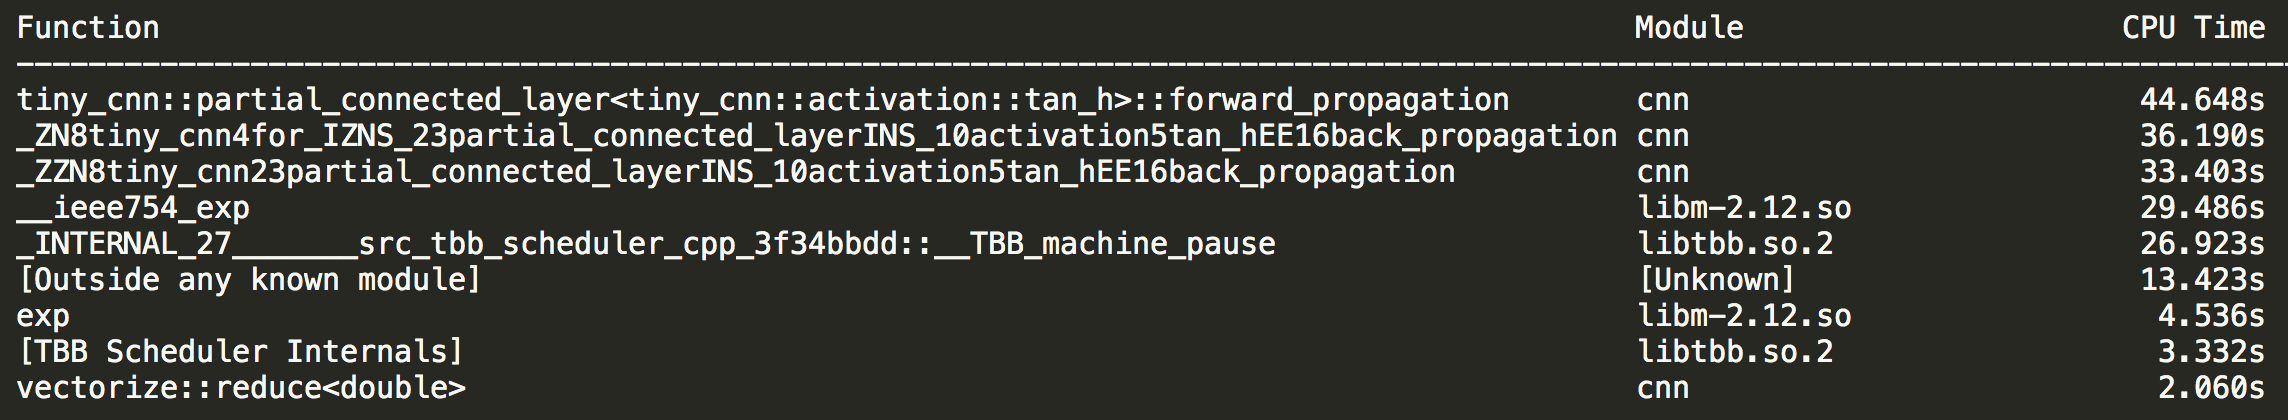
\includegraphics[width=0.9\tw]{fig-profiling.png}

  \caption{\textbf{Profiling results --} Only the top few most expensives functions are shown for brevity.}

  \label{fig-profiling}

\end{figure}


\subsection{Identifying Performance Bottlenecks}

To begin our investigation of Tiny CNN and to guide the direction of our tuning and improvements we began by profiling the author's original implementation which uses TBB (thread building blocks).

Our findings are shown in figure~\ref{fig-profiling}. Forward and backwards propogation take the most time. This is unsurprising as forward propogation and backward propogation consitute the majority of work in determining the label of an example and then determining the gradient at each layer of the neural network.

This suggested to us that we should focus on improving forward propogation and backward propogation. This means improving the code within each layer which is used for forward and backward prop and parallelizing propogation as much as possible. It is possible to parallelize forward and backwards propogation of images as the neural network can be updated at the very end of backwards propogation once all gradients for all images are found.
